\documentclass[11pt]{article}
\usepackage[margin=1in]{geometry}
\usepackage{graphicx}
\usepackage[font=small,labelfont=bf,skip=6pt]{caption}
\usepackage{parskip}
\graphicspath{{figs/}}

\title{Substack piece: final figure lineup\\[2pt]
\large The fine print of event contracts predicts disputes}
\author{}
\date{Locked --- \today}

\begin{document}
\maketitle

\noindent Narrative order: a disaster you could have seen in the text (Fig.~1);
the model works in the real world, unweighted (Fig.~2), and its probabilities
are honest (Fig.~3); how the AI reads a contract (Fig.~4) and which flaws carry
the signal (Fig.~5); the letter grades (Fig.~6). Every statistic is
out-of-sample: markets are scored by a model that never saw their series or
market family.

\begin{figure}[h!]
\centering
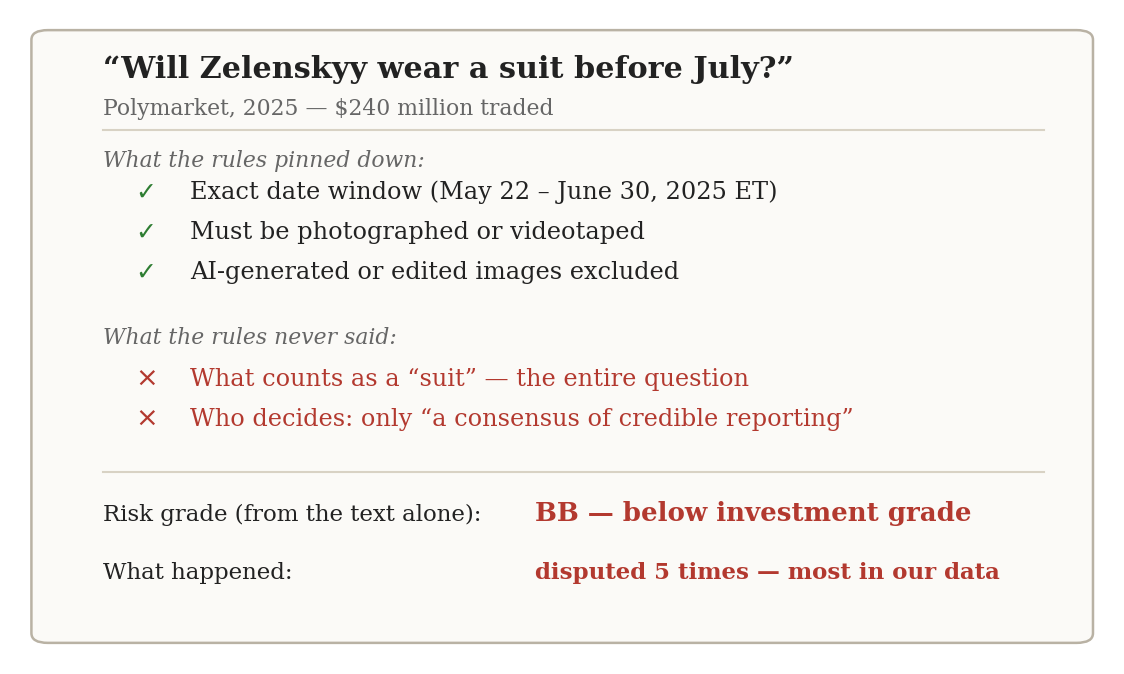
\includegraphics[width=0.86\textwidth]{fig1_contract.png}
\caption{\textbf{The suit market's rules, annotated.} The actual rules of Polymarket's \$240M
Zelenskyy-suit market: precise about the wrong things (dates, deepfakes),
silent on the word the market was named after and on who decides. From the
text alone it grades BB --- below investment grade; scored out-of-sample (by a
model that never saw this market or its siblings) it lands in the riskiest
tenth of Polymarket. In fact it was disputed five times, the most of any
market in the data.}
\end{figure}

\begin{figure}[h!]
\centering
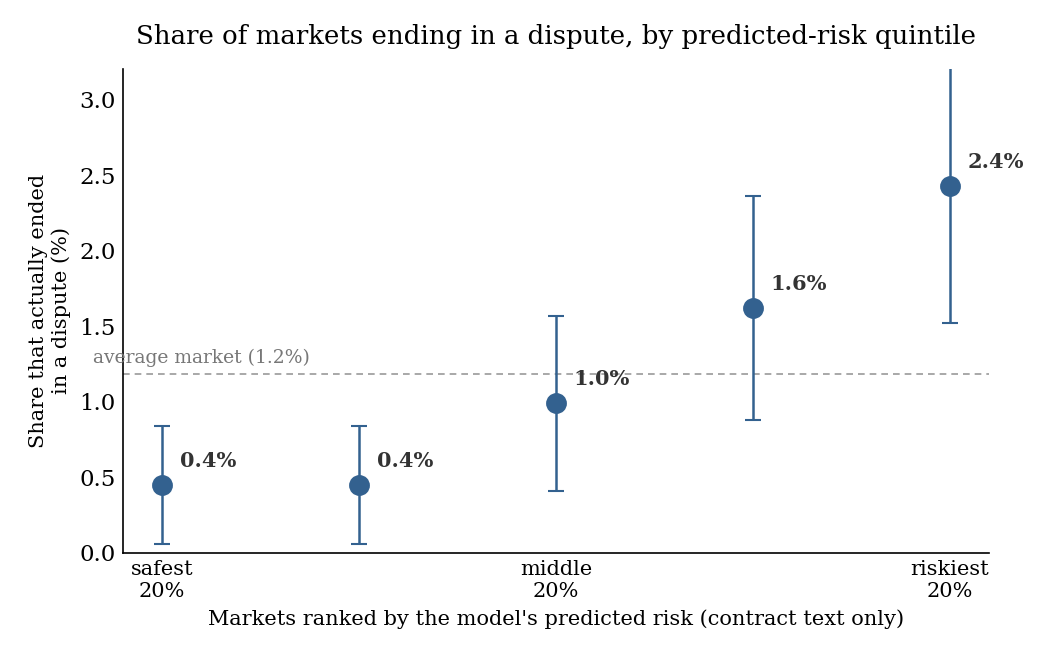
\includegraphics[width=0.9\textwidth]{fig2b_realworld.png}
\caption{\textbf{Real-world dispute rates by predicted-risk quintile.} All 5{,}567 markets in the representative random sample (both
platforms), ranked by the model's predicted risk from contract text alone and
split into quintiles; the y-axis is the raw share that actually ended in a
dispute (95\% binomial CIs). The riskiest fifth disputes at $\sim$6$\times$
the rate of the safest fifth. Companion fact for the text: on Polymarket ---
where disputes are organic third-party challenges, the purest prediction test
--- 6 of the 9 real-world disputes landed in the model's riskiest 20\% of
markets (out-of-sample AUC 0.78).}
\end{figure}

\begin{figure}[h!]
\centering
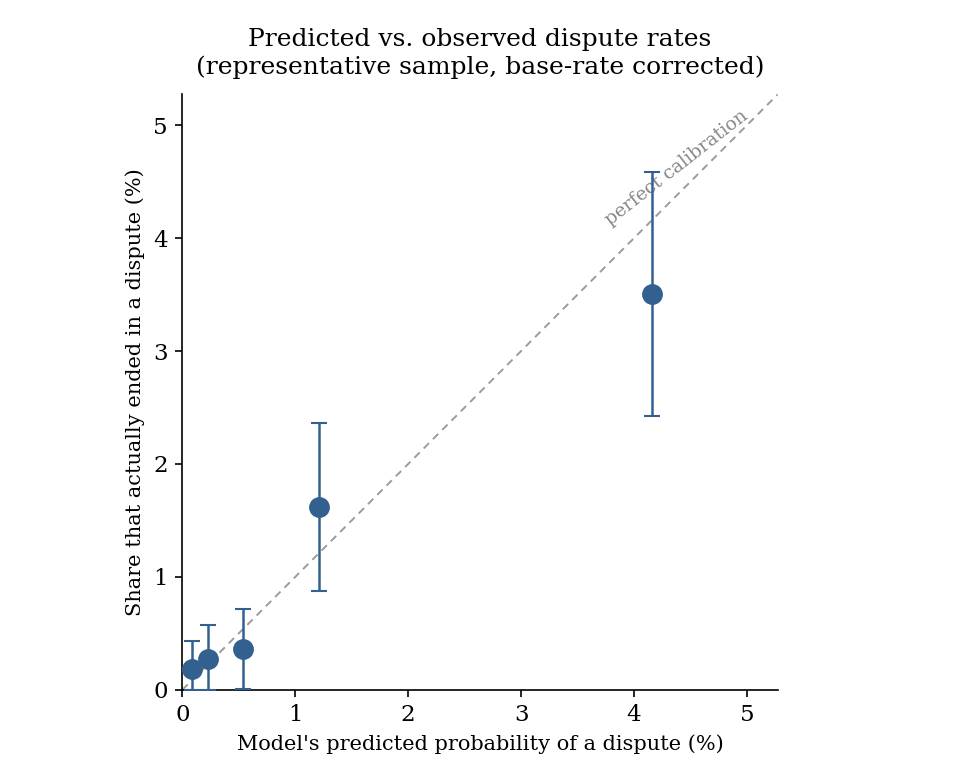
\includegraphics[width=0.68\textwidth]{fig2c_probability.png}
\caption{\textbf{Calibration of the corrected predicted probabilities.} The same out-of-sample
scores converted to real-world probabilities (per-platform base-rate
correction), binned, against the share of markets that actually disputed;
the dashed line is perfect calibration. When the model says $\sim$4\%, about
3.5\% of those markets blow up; every bin's CI crosses the line. The model
doesn't just rank markets correctly --- its numbers mean what they say.}
\end{figure}

\begin{figure}[h!]
\centering
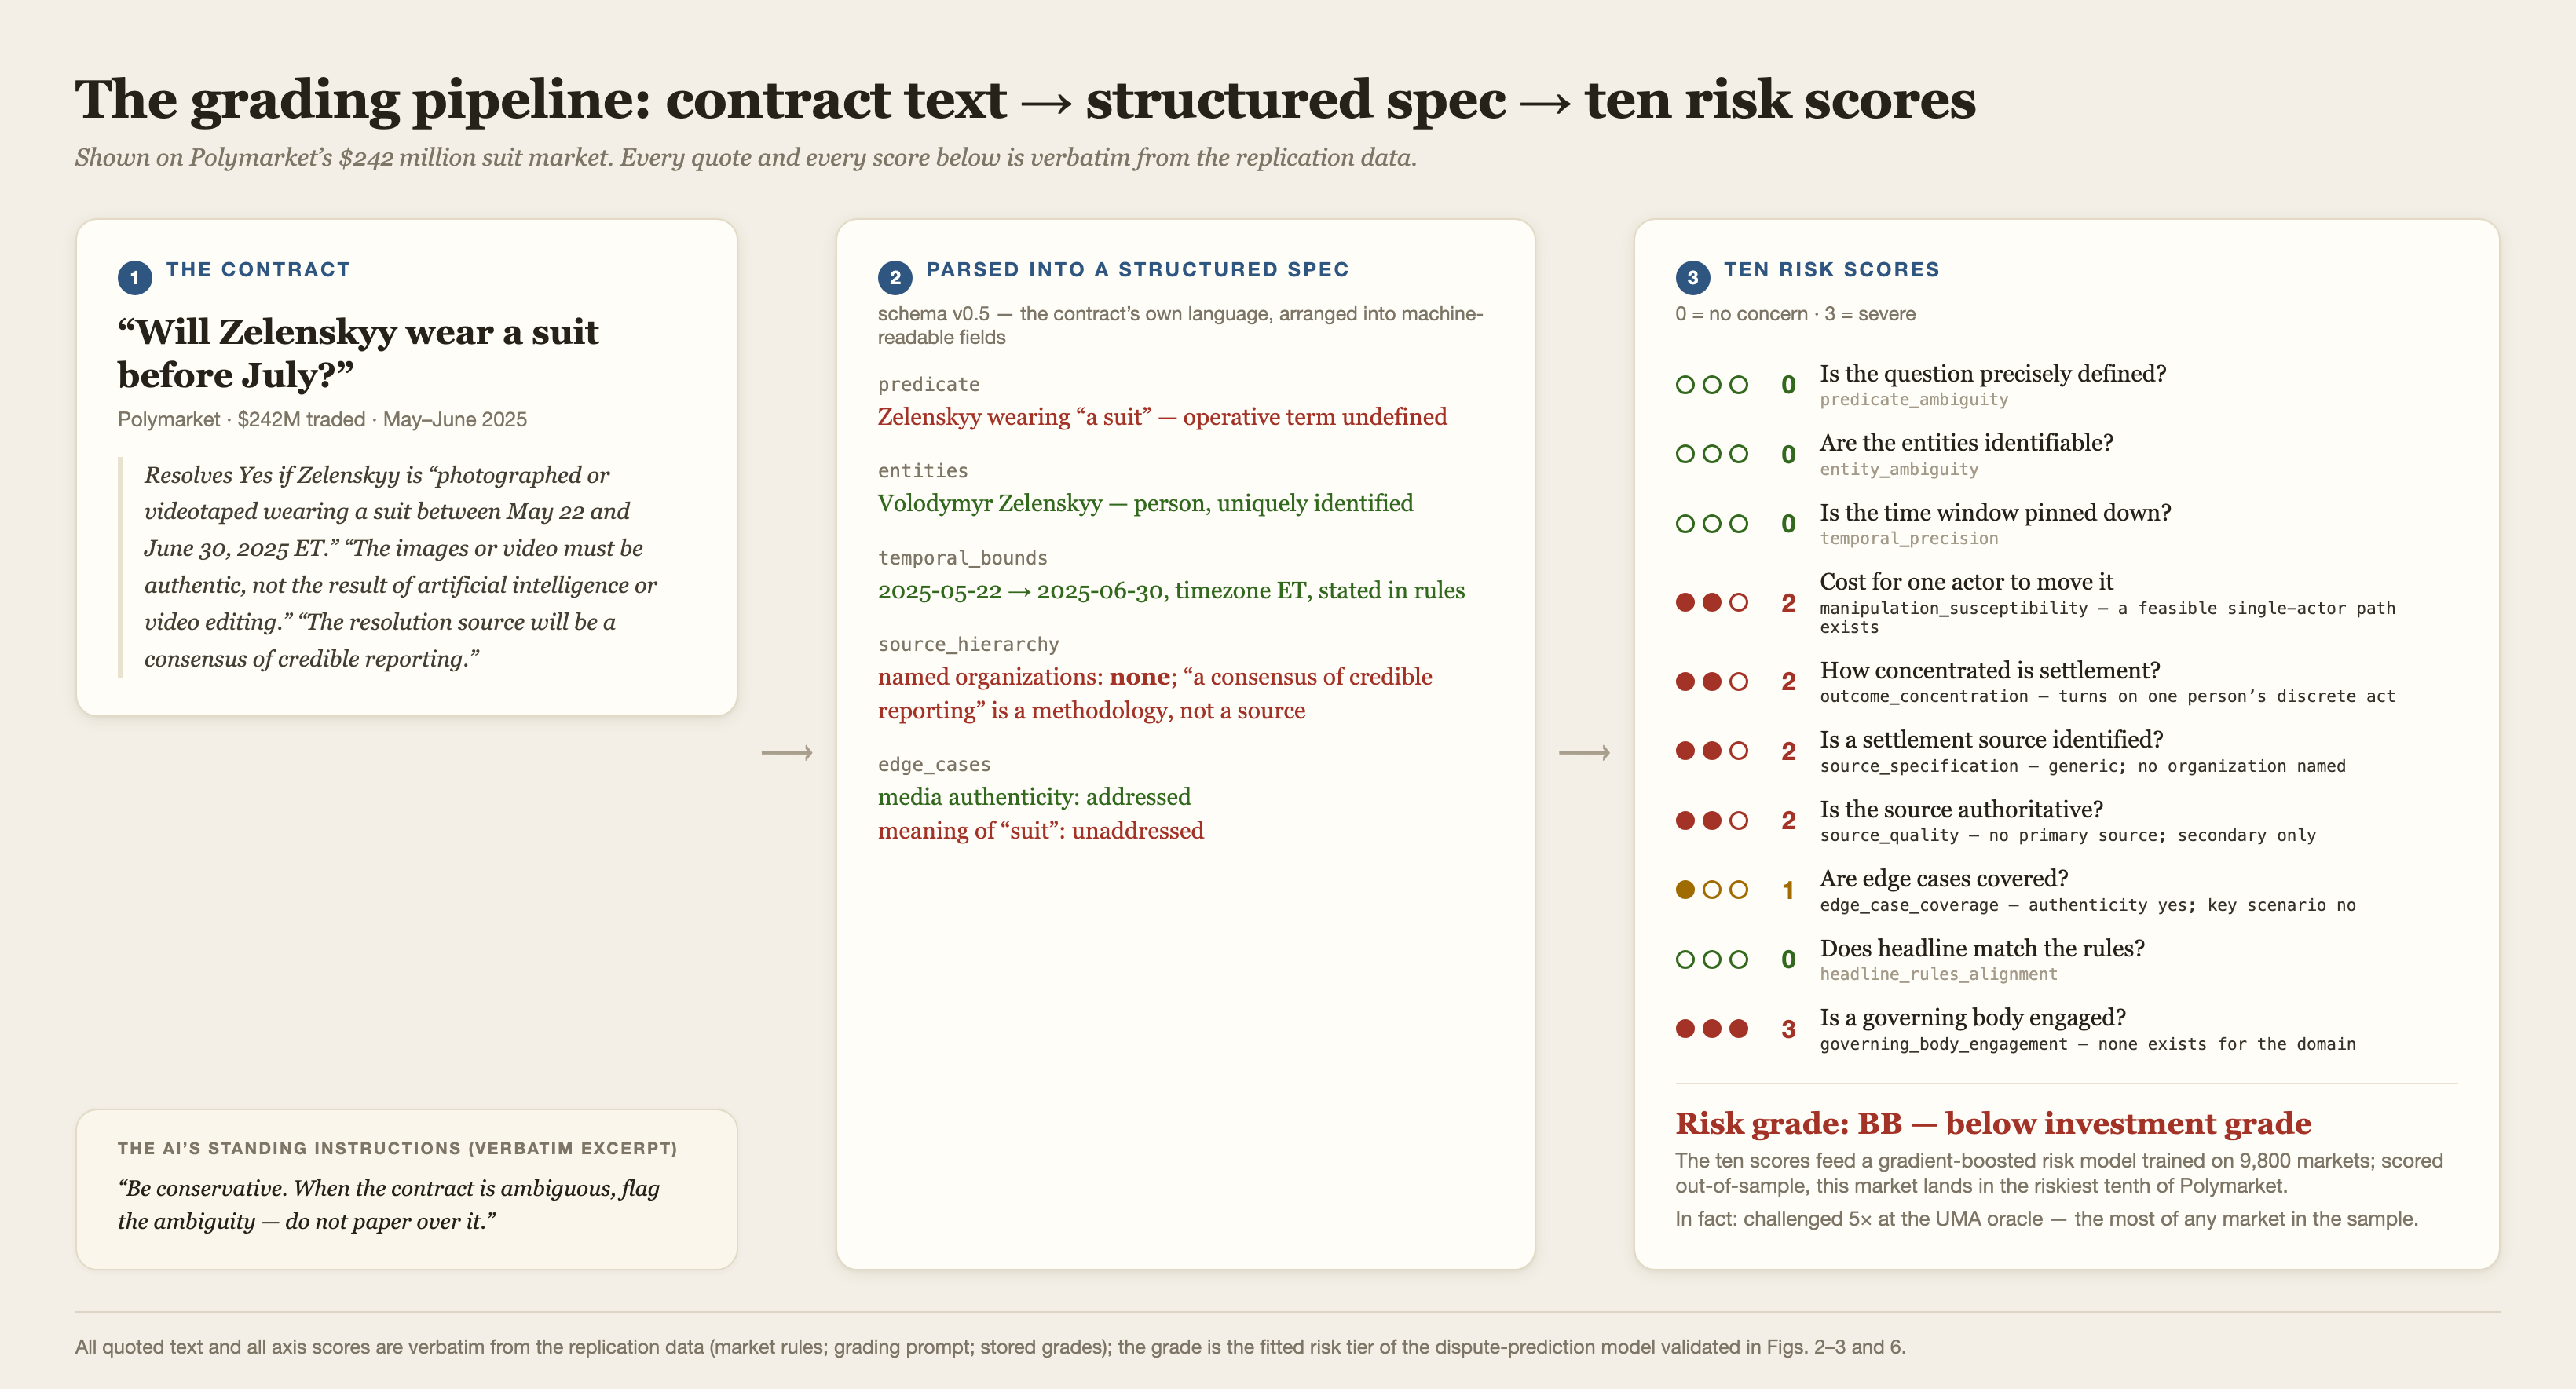
\includegraphics[width=\textwidth]{fig_pipeline_styled.png}
\caption{\textbf{The grading pipeline, applied to one contract.} The pipeline on the suit market
itself. Provenance: the rules text and standing instructions are verbatim
quotes (from the market's oracle record and the actual grading prompt); the
ten axis scores and their schema names are the stored values in the
replication data; step~2 arranges the contract's own language into the real
schema fields (the per-market parse itself is not part of the public data).
The ten scores are the inputs to the gradient-boosted dispute-risk model
validated in Figs.~2--3; the grade (BB, below investment grade) is that
model's fitted risk tier from Fig.~6, and out-of-sample this market's
predicted risk sits in the riskiest tenth of Polymarket. One miss, disclosed: the AI scored the question itself
as precisely defined --- ``suit'' proved otherwise --- yet the missing referee
(no named source, no settling authority, a one-person outcome) pushed the
market below investment grade from the text alone.}
\end{figure}

\begin{figure}[h!]
\centering
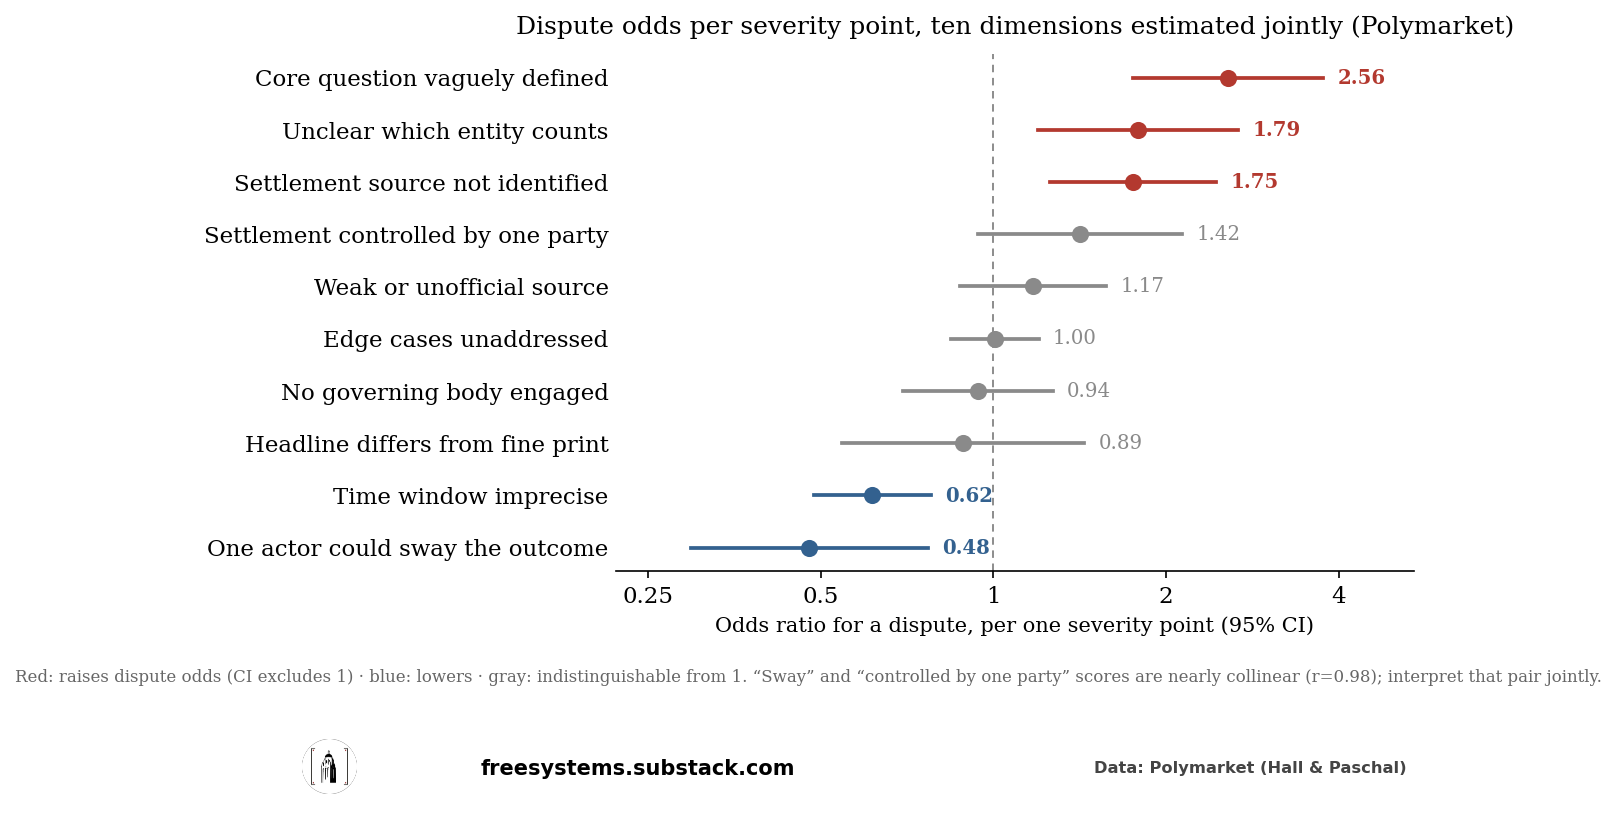
\includegraphics[width=0.98\textwidth]{fig3_flaws.png}
\caption{\textbf{Dispute odds by contract dimension, jointly estimated.} One
logistic regression of the dispute indicator on all ten 0--3 severity scores
at once; Polymarket organic specification disputes vs.\ clean markets
($n=3{,}643$; 877 disputes). Points: odds ratio per one severity point;
whiskers: 95\% CIs clustered by market family. Odds ratios are invariant to
the dispute oversampling, so no level caveat is needed. Vaguely defined core
questions, ambiguous entities, and unidentified settlement sources raise
dispute odds, holding the other dimensions fixed; manipulability and
imprecise time windows lower them (manipulable markets tend to resolve
unambiguously); the remaining dimensions are indistinguishable from no
effect. The two structural scores are nearly collinear ($r=0.98$) and should
be read as a pair. (Kalshi's exchange flags behave differently and are
analyzed separately in the paper.)}
\end{figure}

\begin{figure}[h!]
\centering
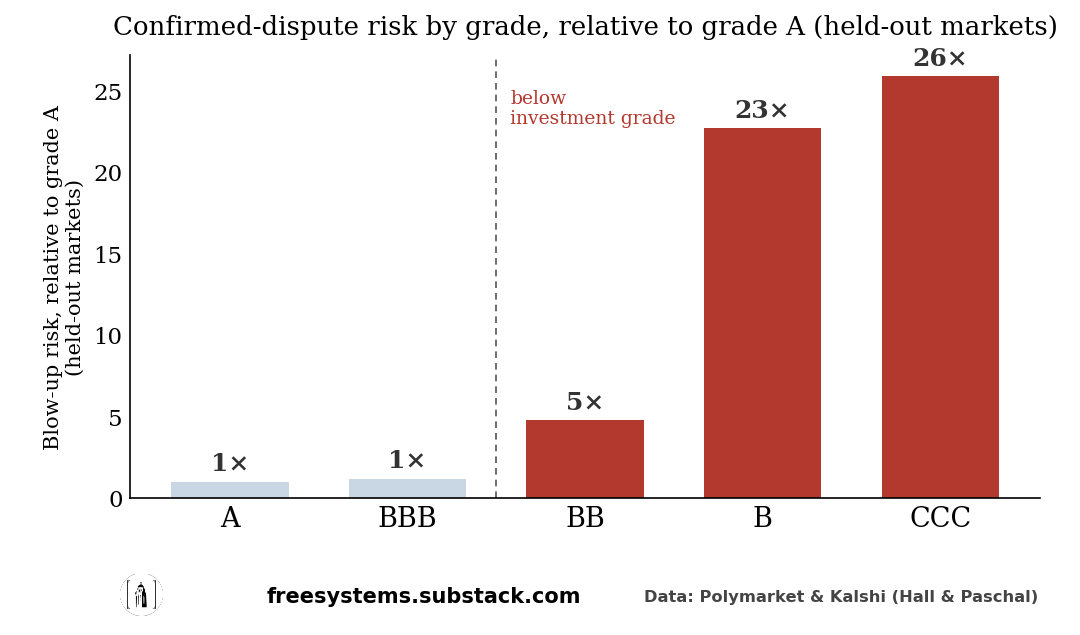
\includegraphics[width=0.82\textwidth]{fig4_grades.png}
\caption{\textbf{Relative dispute risk by grade.} Both platforms, confirmed (demonstrable)
blow-ups, on held-out markets; each grade's risk relative to grade A:
$1\times$, $1.2\times$, $5\times$, $23\times$, $26\times$. A and BBB are
indistinguishable; below the investment-grade line, risk jumps an order of
magnitude. Relative units by design --- absolute blow-up rates are tiny
everywhere (real-world dispute rates are $\sim$0.3--2\%); the grade tells you
the multiplier.}
\end{figure}

\end{document}
